\documentclass{article}
\usepackage{graphicx} % Required for inserting images
\usepackage{float}
\usepackage{polski}
\usepackage[a4paper, top=2cm, right=2cm, bottom=2cm, left=2cm, marginparwidth=1.5cm]{geometry}
\usepackage{amsmath}
\usepackage[export]{adjustbox}
\usepackage{amssymb}
\usepackage{listings}
\usepackage{xcolor}
\usepackage{subcaption}
\usepackage{titlesec}

\titleformat{\section}
  {\normalfont\Large\bfseries}
  {\thesection.}{1em}{}

\titleformat{\subsection}
  {\normalfont\large\bfseries}
  {\thesubsection.}{1em}{}

\titleformat{\subsubsection}
  {\normalfont\normalsize\bfseries}
  {\thesubsubsection.}{1em}{}

\title{Golang}
\author{Michał Witkowski}
\date{Czerwiec 2024}

\begin{document}

\maketitle

\section{Wstęp}

\vspace{1em}

Dokumentacja w formie streszczonej. Opis zawiera zadania, które mamy przesłać, a które nie zostały ocenione.


\section{Zadania}

\subsection{Symulacja spalania lasu}

Symulacja spalania lasu to przede wszystkim wygenerowana tablica tablic (lub inaczej tablica dwuwymiarowa), dla której każdym elementem jest drzewo bądź ziemia. Dodatkowo przy każdym uruchomieniu generowany jest losowy punkt na mapie w który uderza piorun, doprowadzając do spalenia części drzew, w zależności od wiatru jaki wieje oraz gęstości zalesienia.

\vspace{2em}

\lstset{ %
  language=Go,                    % Język programowania
  basicstyle=\ttfamily\small,     % Podstawowy styl tekstu
  keywordstyle=\color{blue},      % Styl dla słów kluczowych
  commentstyle=\color{gray},      % Styl dla komentarzy
  stringstyle=\color{red},        % Styl dla łańcuchów znaków
  numbers=left,                   % Numerowanie linii
  numberstyle=\tiny\color{gray},  % Styl numerowania linii
  stepnumber=1,                   % Co która linia ma być numerowana
  numbersep=5pt,                  % Odstęp numerów linii od kodu
  showspaces=false,               % Pokazywanie spacji
  showstringspaces=false,         % Pokazywanie spacji w łańcuchach
  tabsize=2,                      % Wielkość tabulatora
  breaklines=true,                % Dzielenie długich linii
  breakatwhitespace=false,        % Dzielenie linii tylko na białych znakach
  escapeinside={\%*}{*)}          % Wstawianie LaTeX w kodzie
}

\begin{lstlisting}
func main() {
	forestSize := 100 //best size for the forest
	density := 0.4

	fmt.Println("Welcome to the Burning Forest simulation!")

	forest := CreateForest(forestSize, density)

	fmt.Println("What a peaceful day we have in here:")
	VisualizeForestInConsole(forest)
	fmt.Println("Image is being saved...")
	VisualizeForestOnImage(forest, 100, "data/forest-before.png")

	lightning_x := rand.Intn(forestSize)
	lightning_y := rand.Intn(forestSize)
	forest.SpreadFireWithWind(lightning_x, lightning_y, "W")
	fmt.Printf("Not for long! The lightning strikes at (%d, %d)!\n", lightning_x, lightning_y)

	fmt.Println("The forest after burning:")
	VisualizeForestInConsole(forest)
	fmt.Println("Image is being saved...")
	VisualizeForestOnImage(forest, 100, "data/forest-after.png")

	// percentage of burnt trees
	burntPercentage := calculatePercentageOfBurntTrees(forest, forestSize)
	fmt.Printf("%.2f%% of the forest got burned.\n", burntPercentage)

	// optimal density
	fmt.Println()
	numberOfSamples := 1000
	// caution - it takes a while to calculate the optimal density
	optimalDensityForDefault := findOptimalDensity(forestSize, numberOfSamples)
	optimalDensityForNorth := findOptimalDensityForNorth(forestSize, numberOfSamples)
	optimalDensityForEast := findOptimalDensityForEast(forestSize, numberOfSamples)
	optimalDensityForWest := findOptimalDensityForWest(forestSize, numberOfSamples)
	optimalDensityForSouth := findOptimalDensityForSouth(forestSize, numberOfSamples)

	fmt.Printf("Optimal density for fire without any wind is %.2f%%.\n", optimalDensityForDefault*100)
	fmt.Printf("Optimal density for fire during nothern wind is %.2f%%.\n", optimalDensityForNorth*100)
	fmt.Printf("Optimal density for fire during eastern wind is %.2f%%.\n", optimalDensityForEast*100)
	fmt.Printf("Optimal density for fire during western wind is %.2f%%.\n", optimalDensityForWest*100)
	fmt.Printf("Optimal density for fire during southern wind is %.2f%%.\n", optimalDensityForSouth*100)

	optimalDensities := map[string]float64{
		"No Wind": optimalDensityForDefault * 100,
		"North":   optimalDensityForNorth * 100,
		"East":    optimalDensityForEast * 100,
		"West":    optimalDensityForWest * 100,
		"South":   optimalDensityForSouth * 100,
	}

	createBarChart(optimalDensities, "data/bestDens.png")
}

\end{lstlisting}

\vspace{2em}

Kod w skrócie opisuje, jak działa program, tworzymy las, wizualizujemy go zarówno w konsoli jak i za pomocą obrazu, wywołujemt pożar a następnie wizualizujemy skutki tego pożaru dla odpowiednich parametrów.
Na koniec w formie analizy sprawdzamy, jaka byłaby odpowiednia gęstość zalesienia, by zminimalizować straty (wyniki wysokie dla testów z wiatrem mogą być pochodną faktu, że wiatr zawieje ogień tak, by procentowo las spłonął w takim samym stopniu, nie ważne od zalesienia).

\vspace{2em}

\begin{figure}[h]
  \centering
  \begin{subfigure}[t]{0.48\textwidth}
    \centering
    \includegraphics[width=\textwidth]{photos/forest-before.png}
    \caption{Las przed spaleniem}
  \end{subfigure}%
  \hfill
  \begin{subfigure}[t]{0.48\textwidth}
    \centering
    \includegraphics[width=\textwidth]{photos/forest-after.png}
    \caption{Las po spaleniu}
  \end{subfigure}
\end{figure}

\vspace{2em}

Naszym wynikiem wtedy są wygenerowane obrazy lasu sprzed oraz lasu po spaleniu

\vspace{2em}

Oprócz tego w naszym lesie jest jeszcze troche obliczeń. Między innymi jest to obliczanie optymalnego zalesienia dla lasu tak, aby las przetrwał w jak najlepszym stanie. Wykonujemy to na 1000 próbkach, czyli wykonaniu symulacji 1000 razy na różnych stopniach zalesienia i wyciągnięcie z tego średniej wartości.

\vspace{1em}

To co wylicza nam program możemy zobaczyć na przedstawionym grafie.

\vspace{2em}

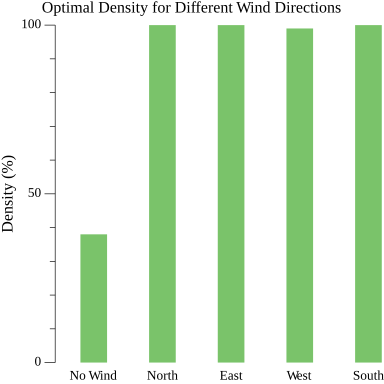
\includegraphics[width=25em, height=25em, center]{photos/bestDens.png}


\vspace{2em}

\subsection{Prosty serwer z danymi ataku rekinów}

Innym zadaniem jest zrobiony serwer http przy użyciu biblioteki "net/http" oraz frameworka Gin. Prosty serwer łączy się z bazą danych, którą w tym przypadku jest nasz plik json i umożliwia nam pokazanie 10 losowych postów, usunięcie posta po odpowiednim id, aktualizację posta.

\begin{itemize}
    \item GET /shark - zwraca nam 10 losowych postów
    \item POST /shark - mozemy dodac własny Post, w odpowiednim formacie json
    \item DELETE /shark/id - usuwamy Post o danym id
    \item PUT /shark/id - mozemy zaktualizowac obiekt o podanym id
\end{itemize}

Testy wykonywane przy użyciu Postmana (narzędzie to wysyłania zapytań na endpointy).

\subsection{Szyfr Cezara oraz szyfr afiniczny}

Jednym z zadań jakie robiłem był szyfr cezara oraz szyfr afiniczny zrobiony w Go. Przyjemny program, który odpowiadał za szyfrowanie tesktu według klucza, odszyfrowywanie go oraz znajdywanie klucza metodą szukania.


\subsection{Inne mniejsze zadanka}

\subsubsection{Colatz}

Z innych zadań mamy zadanko z problemem colatza, które polega na tym, żę sprawdzamy X liczb i czy dla nich kroki:
\begin{itemize}
    \item Jeśli liczba jest parzysta, podziel ją przez 2.
    \item Jeśli liczba jest nieparzysta, pomnóż ją przez 3 i dodaj 1.
    \item Powtarzaj te kroki dla nowej liczby.
\end{itemize}

Wg tego schematu, zawsze dojdziemy do 1. No właśnie, ale czy zawsze? Na tym polega ten problem, nie można udowodnić, że dla każdej liczby wynik końcowy bedzie 1.


\subsubsection{Wykrywanie prawidłowości numeru PESEL}

Kolejne zadanko to prosta zabawa z regułami wg których robione są pesele. Dzięki temu mamy prostą "sprawdzarkę", czy pesel jest prawdziwy

\subsubsection{Zadanko na wyliczanie odległości punktu (X,Y)}

Krótkie zadanko polegające na zrozumieniu i docenieniu wartości typów generycznych. Obliczanie odległości Punktu(X,Y) od punktu(0,0).

\subsubsection{Matrix}

Prosta zabawa na macierzach.

\section{Zakończenie}

Moja propozycja na ocenę końcową z przedmiotu to 4.5. Usprawiedliwieniem tej oceny są powyższe projekty, które pokazują moje zaangażowanie w przedmiot oraz chęć do samodzielnej pracy. Dodatkowo od siebie mogę dodać, że reprezentując uczelnię w tym tygodniu na Woman In Tech Summit 2024 miałem okazję użyć wiedzy z go nabytej na Twoim przedmiocie w rozmowach z rekruterami, którzy się tam znajdowali. Nie jest to co prawda stricte praca na zajęciach, natomiast myślę, że dobrze wpasowuje się w Twoją chęć, byśmy zgłębiali i wykorzystywali język na własną rękę, a nie tylko "z przymusu narzuconych zadań".

\end{document}
